
\chapter{Data analytics}

In this chapter I propose three hypotheses. They are:

\begin{enumerate}
  \item Skedge's differences from and additions to CDCS are \textbf{usable and have real need}.

  \item Skedge’s \emph{navigations-per-add} demonstrate the \textbf{effectiveness of its search features} for each of the following three user search paradigms:

  \begin{enumerate}
    \item direct search,
    \item exploratory search, and
    \item peer-guided search
  \end{enumerate}

  \item \textbf{SkedgeQL is user-friendly}; users learn how to make more sophisticated search queries over time \textbf{simply by using it}.
\end{enumerate}

\noindent In the following sections I will present my analysis on collected usage data since November 3rd 2015, which will serve to validate each hypothesis.

\section{Usage}

\subsection{General}

From November 3, 2015 to April 11, 2016 (a period of 159 days), Skedge has seen\ldots

\begin{itemize}
  \item 4,713 users that have added or bookmarked at least one course
  \item 5,256 schedules
  \item 17,124 sessions\footnote{A session is defined by a period of activity expiring after 30 minutes of inactivity}, 75\% of which are from returning visitors
  \item an average of 107 sessions per day
  \item an average of 5.4 pages viewed per session 
  \item an average of 6 minutes spent per session
\end{itemize}

\subsection{Search}

\begin{figure}[H]
  \centering

  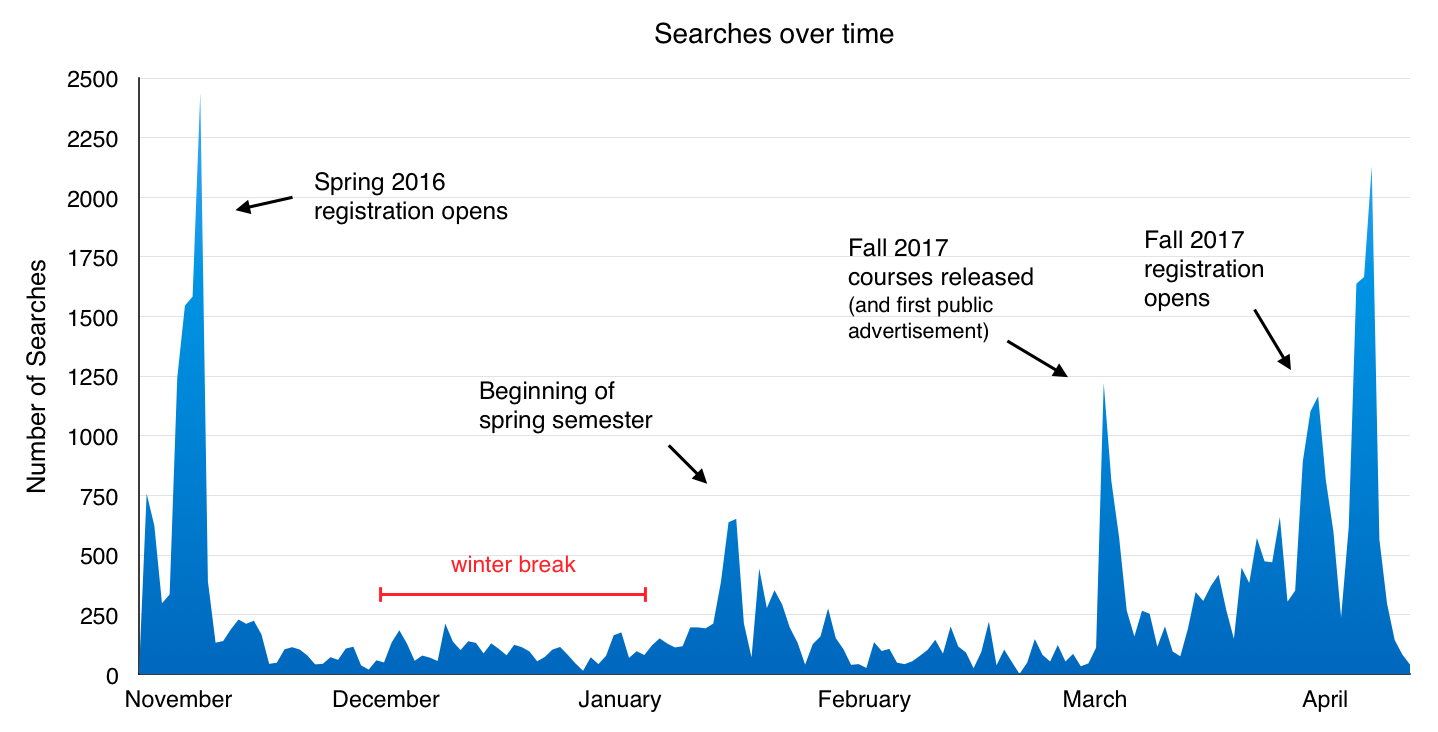
\includegraphics[width=1.0\textwidth]{images/graph/searches}

  \caption{Searches over time, with major relevant calendar events annotated}
  \label{fig:searches}

\end{figure}

Figure \ref{fig:searches} shows user search submissions over the time, and makes the periodicity of Skedge usage extremely apparent. Although it only shows a bit more than one ``phase,'' the cycle of events---\emph{semester begins} (students check course times, room locations, etc. while they get accustomed to the semester), \emph{next semester's course catalog released} (students explore the courses offered and build possible schedules), \emph{next semester registration opens} (cross-checking and officially registering each course with the Registrar)---clearly drives the majority of site traffic.

What this means is that Skedge is not seen as an experiment or a proof of concept that is not production-ready. Rather, its traffic patterns show that it is consistenly \emph{relied upon} by students and used for its intended purpose in times of biggest course scheduling need. %, and the same can be seen with other usage measures such as schedule exporting and clicking on the Wikipedia-style embedded links (Figures \ref{fig:exports} and \ref{fig:linksearches}, respectively).

It should also be noted that before March, the majority of the userbase as I knew it consisted of seniors, as the majority of people that I knew personally and shared Skedge with belonged to my class. The latest two major events reported in the graph above thus very impressively consist of \emph{very few seniors}, who have no courses left to schedule. March also marked the very first time I publicly advertised Skedge, although not very strongly. It was sent out to all students in the Computer Science mailing list as well as posted to two class-wide Facebook groups.

The usability of and user satisfaction with a tool is hard to measure when it holds a monopoly. Considering that Skedge is an \emph{optional alternative} to CDCS, such consistent usage data (especially with 75\% of sessions being from returning users) undeniably prove its measures of usability and user satisfaction relative to CDCS.


  \subsubsection{Search types}

  \begin{figure}[H]
    \centering
    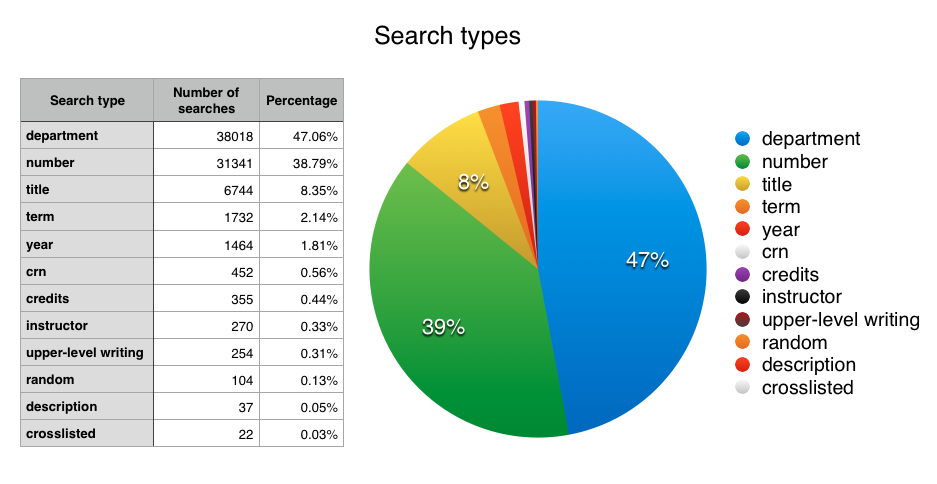
\includegraphics[width=1.0\textwidth]{images/graph/searchtypes}

    \caption{Breakdown of search queries by type of search}
    \label{fig:searchtypes}
  \end{figure}


Figure \ref{fig:searchtypes} validates the hypothesis made in Section 2.3 regarding the search interface design, demonstrating that the \emph{department code} and \emph{course number} search modes dominate user searches, accounting for over 85\% of all searches on Skedge. With this knowledge, bringing out the tucked-away, nondistinct field for this search in CDCS into prominence is a usability design choice that accomodates empirical usage.

\subsubsection{Empty searches}

  Of the total 45,466 searches on Skedge logged since November 2nd 2015, 89.4\% (40,625) of searches produce nonempty search results, whereas 10.6\% (4,841) of searches come up empty. This already is evidence of an effective search mechanism, but of those empty searches, the vast majority

  Can learn from these searches. This is the same method WolframAlpha describes its team using to improve their freeform input system \cite{wolfram2}.

  \begin{figure}
  {\renewcommand{\arraystretch}{1.5}
  \centering
  \begin{tabular}{ p{6cm} p{7.5cm} }
  \hline

    ``{\tt Prereq 280}'' \newline ``{\tt has-Prereq: 280}''
    & Course dependencies \\ \hline

    ``{\tt tuesday 3:25-4:40}'' \newline ``{\tt TR 3:25-4:40}'' \newline ``{\tt m/w}'' \newline ``{\tt classes tuesdays and thursdays between 11:05 and 12:20}'' \newline ``{\tt weekend summer 2016}''
    & \parbox[c]{\hsize}{Better day-of-the-week handling} \\ \hline

    ``{\tt 2 credits natural science}'' 
    & Search by division (although there were very few) \\ \hline

    ``{\tt religion and classics}'' \newline ``{\tt studio art}'' 
    & Search by full department name \\ \hline

    ``{\tt new csc courses}'' 
    & The word ``{\tt courses}'' (somewhat common) \\ \hline

    ``{\tt guo}'' 
    & Instructor without ``{\tt taught by}'' (very common) \\ \hline

    ``{\tt stt212 vs mth201}'' \newline ``{\tt stt212 OR mth201}'' 
    & Searching multiple queries at the same time \\ \hline

    ``{\tt crosslisted csc lin}'' 
    & Probably a more reasonable syntax than the current SkedgeQL one (``{\tt csc x lin}'') \\ \hline

    ``{\tt place: hubbell}'' \newline ``{\tt hubbell friday}'' 
    & Search by location, although motives unclear \\ \hline

    ``{\tt MTH 2*}'' 
    & Using ``{\tt *}'' instead of an omission (e.g. ``{\tt MTH 2}'' would work) \\ \hline

    \hline
  \end{tabular}
  \caption{Example of search queries that produced no results but that indicate demand for added search features. The corresponding features that currently lack in SkedgeQL are described on the right.}
  \end{figure}

\begin{figure}
  {\renewcommand{\arraystretch}{1.5}
  \centering
  \begin{tabular}{ | p{4cm} | p{4cm} | p{4cm} | }
  \hline

    ``{\tt Larry david}''
    & ``{\tt taught by seligman}''
    & ``{\tt cool stuff}''
    \\ \hline

    ``{\tt game of thrones}''
    & ``{\tt fun classes}''
    & ``{\tt fun classes in csc}''
    \\ \hline
    

    ``{\tt easy A}''
    & ``{\tt flute birdman}''
    & ``{\tt how do i make a new schedule}''
    \\ \hline

    \hline
  \end{tabular}
  \caption{Humerous search submissions}
  \end{figure}

\subsection{Exports}

\begin{figure}[H]
  \centering
  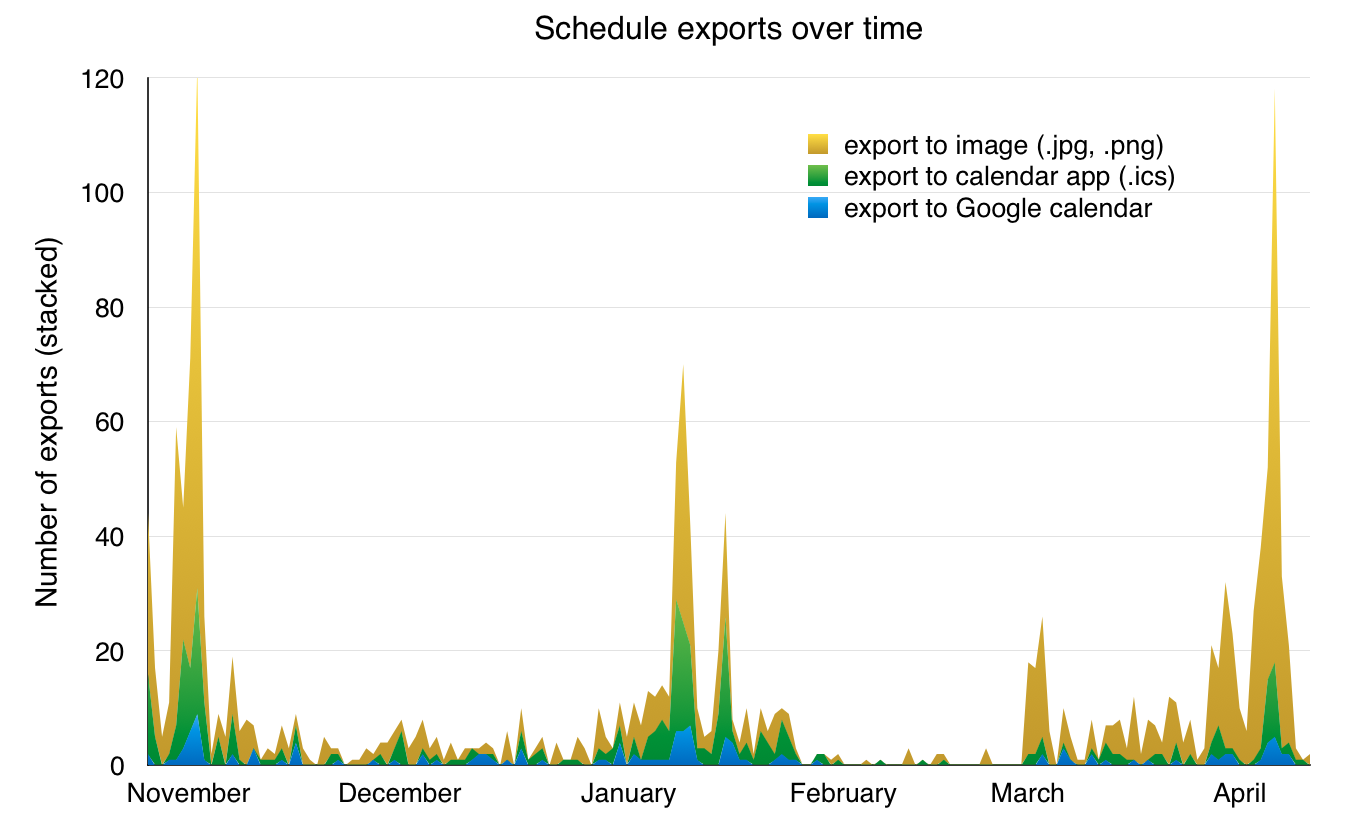
\includegraphics[width=1.0\textwidth]{images/graph/exports}

  \caption{Etc}
  \label{fig:exports}
\end{figure}

Success! (broken on cdcs)

\subsection{``Link-searches''}

\begin{figure}
  \centering
  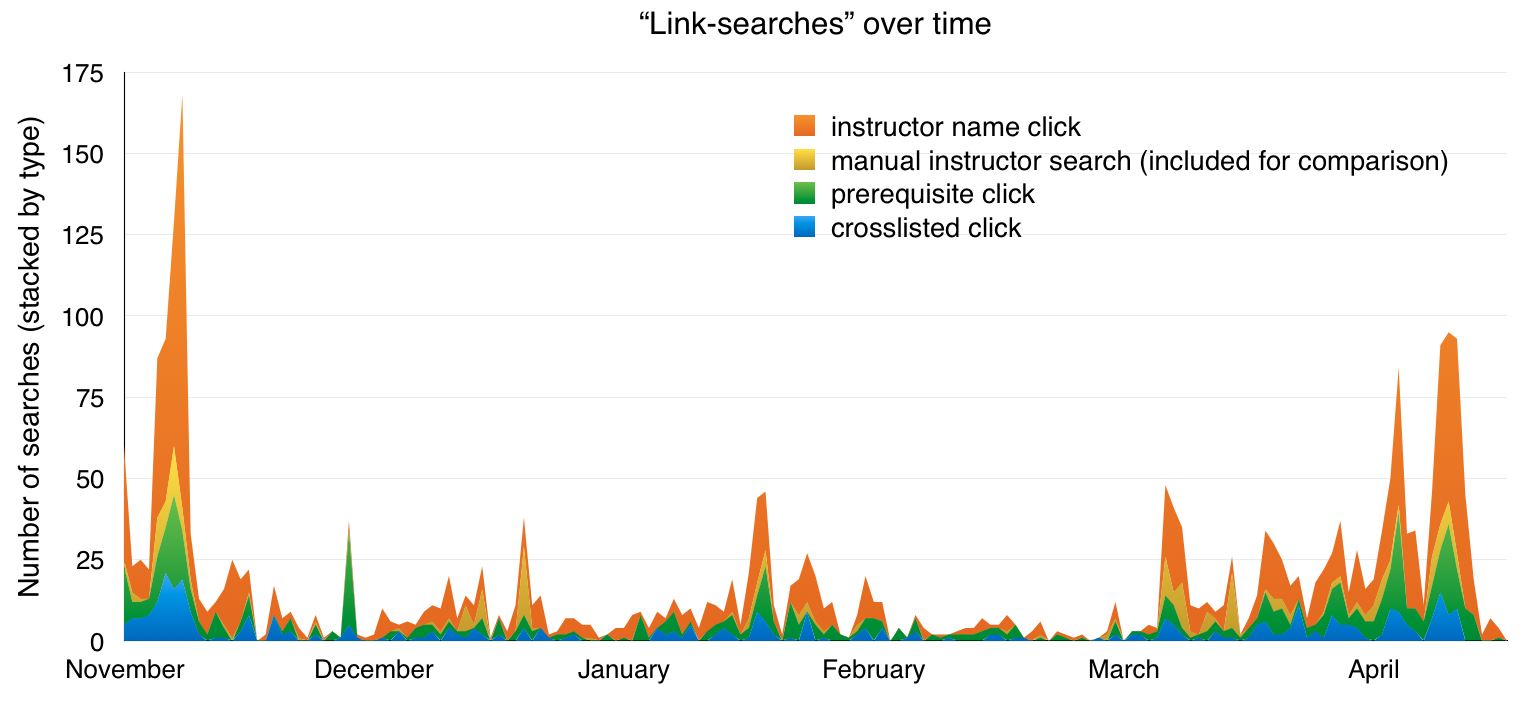
\includegraphics[width=1.0\textwidth]{images/graph/linksearches}

  \caption{Etc}
  \label{fig:linksearches}
\end{figure}

Success, used!

\subsection{Mobile}

\begin{itemize}
  \item 11.54\% of sessions
  \item 2.74 page viewed per session, on average
  \item 2 minutes spent per session, on average
\end{itemize}

success bc mobile doesn't exist on cdcs

\subsection{Course Blocks}

\begin{figure}
  \centering

  \fbox {
    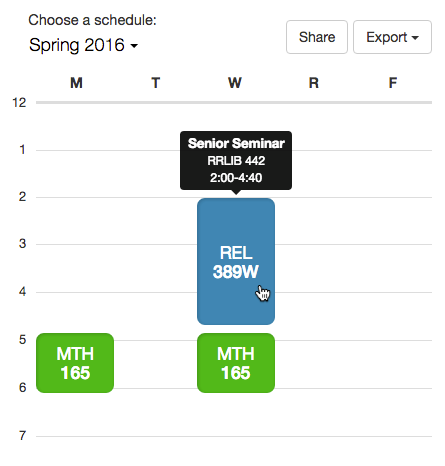
\includegraphics[width=8cm]{images/skedge/blocks}
  }

  \caption{Etc}
  \label{fig:searchtypes}

\end{figure}

40\% of sessions have at least one block-click
Average of 5.12 block-clicks per session

success because you can't click schedule blocks in better cdcs!!

\section{Effectiveness of search}

\subsection{Definitions}

A navigation is defined as
a search, or
a click on an instructor’s name, or
a click on a crosslisted or prerequisite course link

The navigations-per-add measure is
the number of navigations a user took (within one session) until a course was added, bookmarked

\subsection{Trends}

\begin{figure}
  \centering
  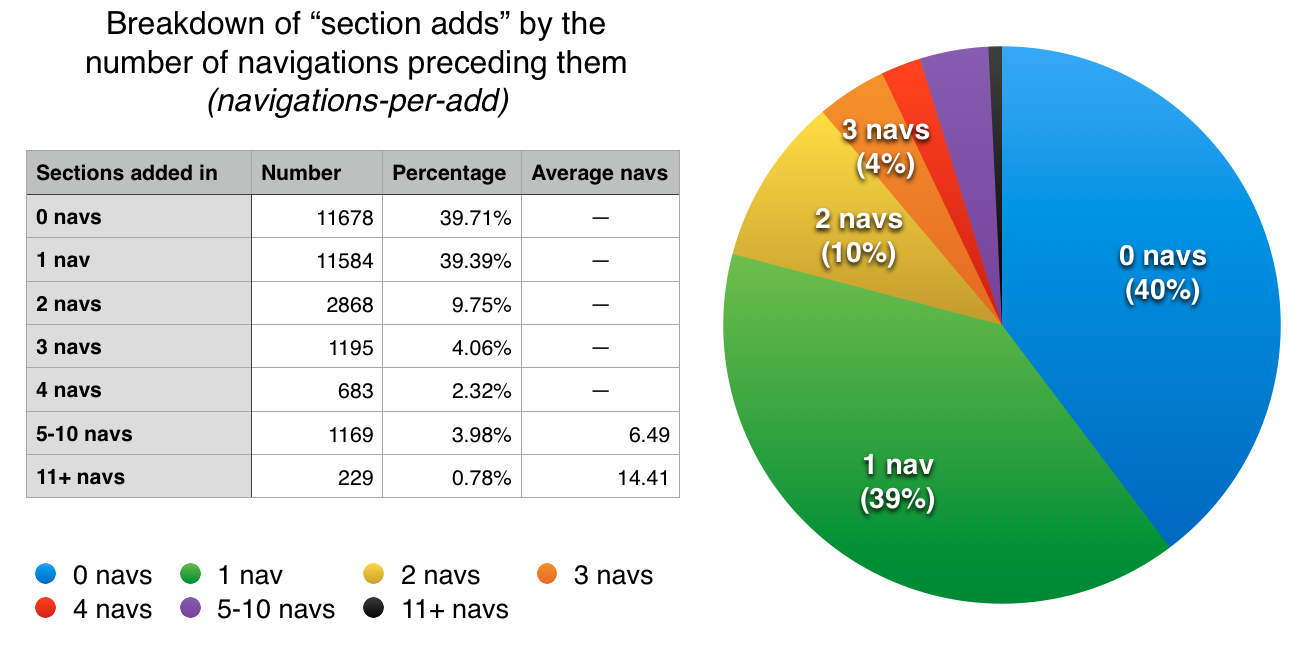
\includegraphics[width=1.0\textwidth]{images/graph/combined_navs}

  \caption{Etc}
  \label{fig:searchtypes}
\end{figure}

\subsection{Breaking them apart}

  behavioral patterns
  Direct search for specific course
  Discovery, browsing, exploring

  \subsubsection{Direct searches}

  \begin{figure}
    \centering
    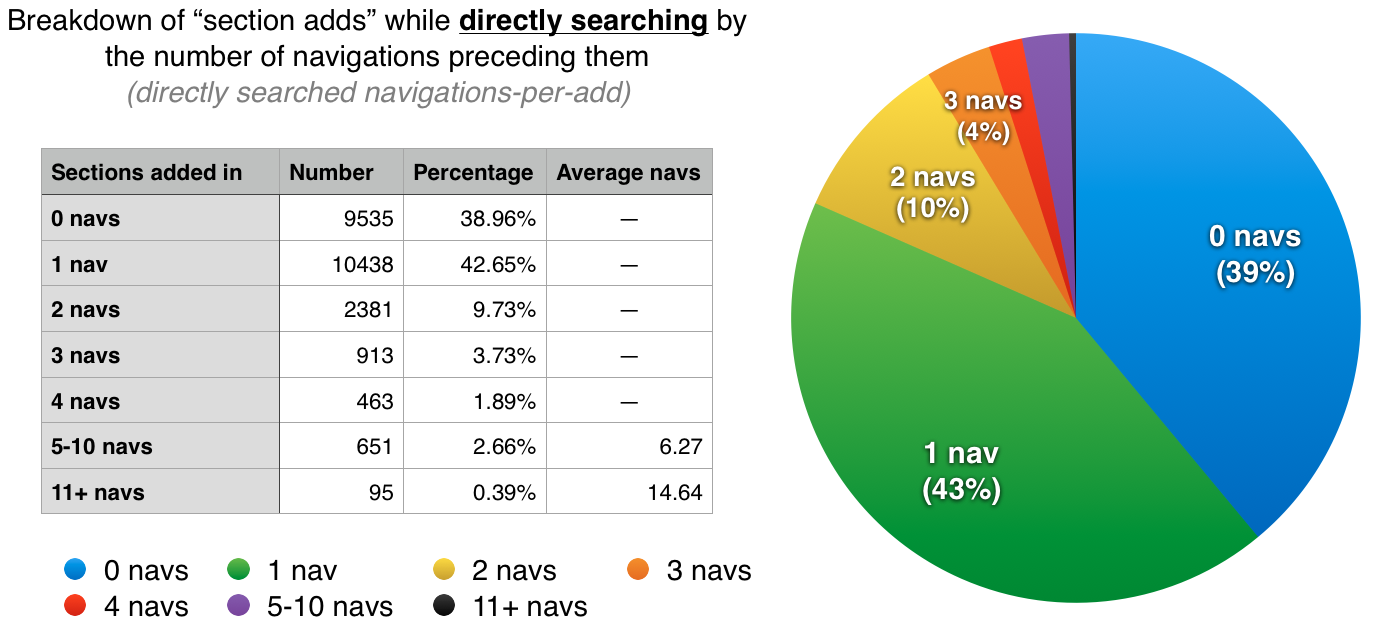
\includegraphics[width=1.0\textwidth]{images/graph/direct_navs}

    \caption{Etc}
    \label{fig:searchtypes}
  \end{figure}

  Why would 0-navs be so common with direct searches? 64\% of them subsections!

  \subsubsection{Browse}

  \begin{figure}
    \centering
    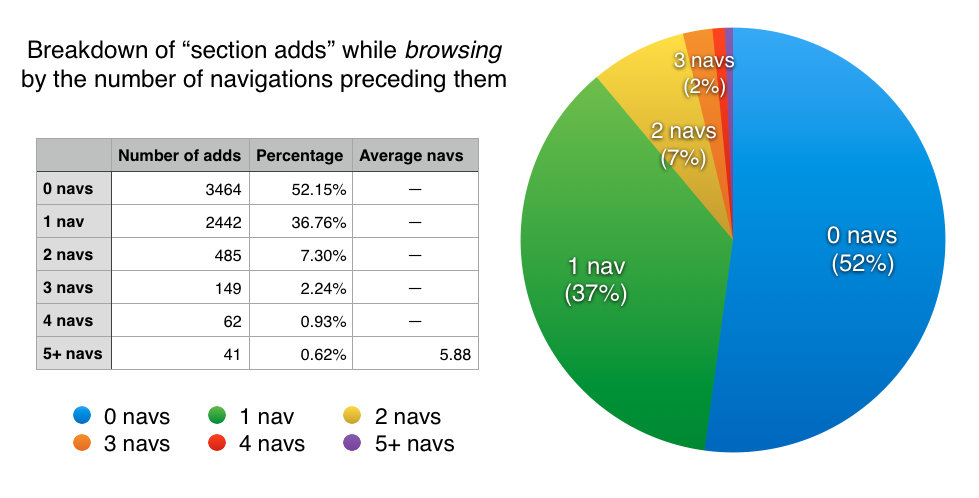
\includegraphics[width=1.0\textwidth]{images/graph/browse_navs}

    \caption{Etc}
    \label{fig:searchtypes}
  \end{figure}

  As expected, the 0-navs were mostly maincourses (62\%)

  Effective++

  \subsubsection{Social}

  90 users have linked Skedge to Facebook
  Since March 1st,
  4,000+ visits (200 visits/day)
  ~60\% of visits to /social were returning visitors
  90 overlays onto friends’ schedules
  10 clicks to Facebook profiles :(
  - get stats from the fb dashboard

  success?????


\section{Complexity of users' searches over time}

\subsection{Definitions}

Points for search by (omits number and dept.):

description
credits
crosslisted
CRN
instructor
title
year
term
‘random’
upper-level writing

“CSC” → 0
“MTH 165” → 0
“taught by hema” → 1   ✓    (2 searches) 
“random mur 1-2 credits” → 2   ✓    (1 search) 


\subsection{Trends}

\begin{figure}
  \centering

  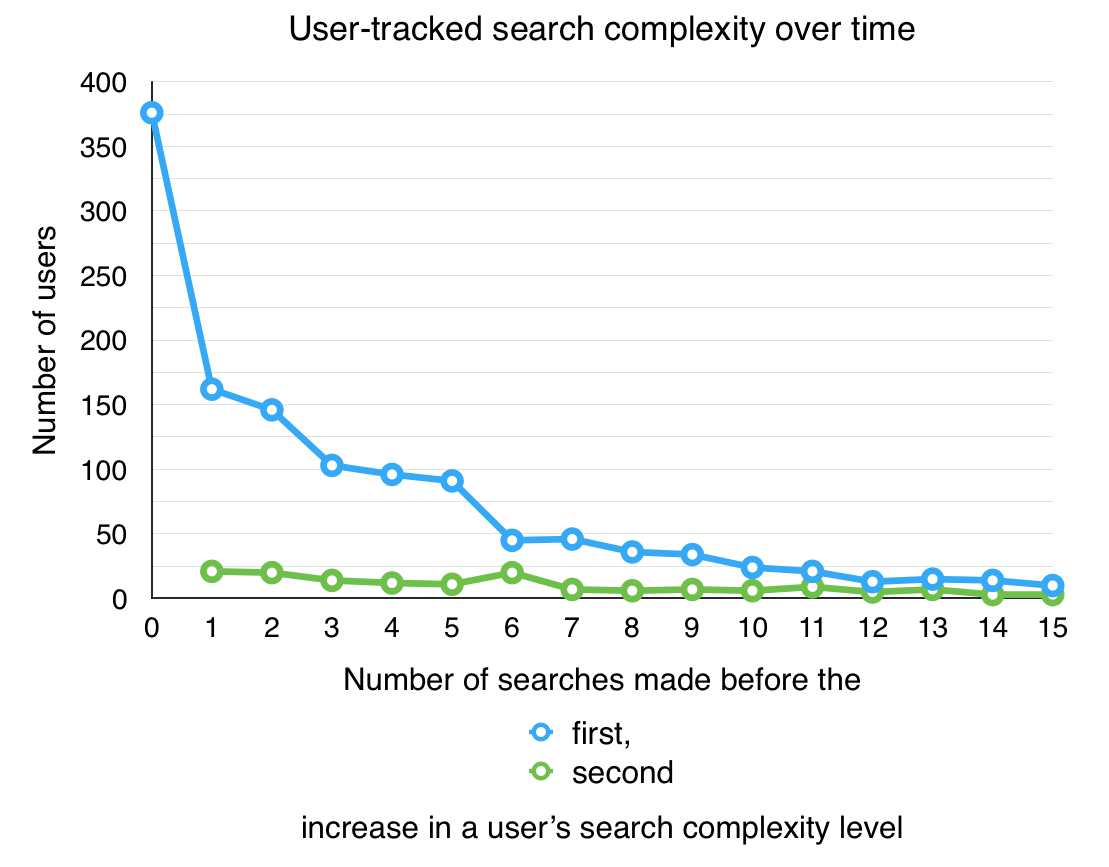
\includegraphics[width=1.00\textwidth]{images/graph/search_dt}

  \\
  \vspace{5pt}

  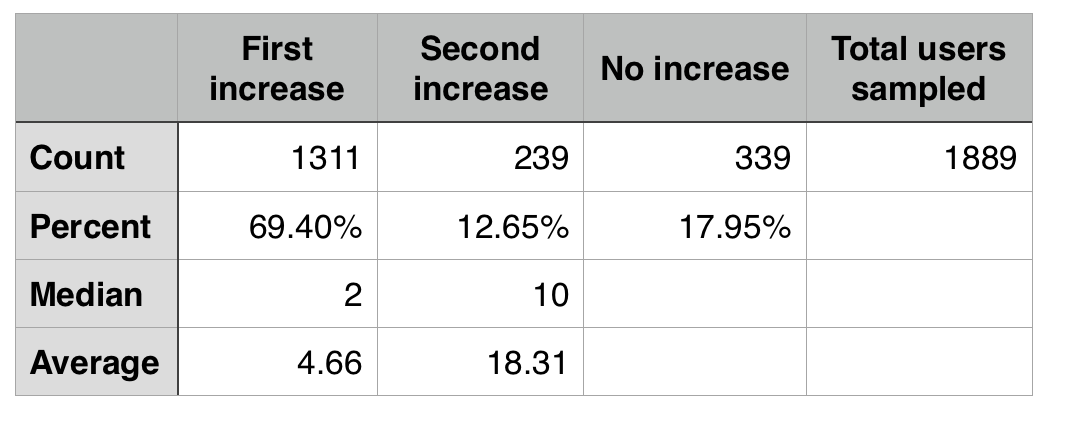
\includegraphics[width=0.65\textwidth]{images/table/search_dt}

  \caption{Etc}
  \label{fig:searchtypes}
\end{figure}

First increase 69.4\% of users), with a median of 2 searches.
Note that starting at search complexity one or greater counts as a ``searches before first increase value'' of 0.

Second increase (7.9\% of users)
Median: 8 searches
Average: 17.52 searches

DSQL++